As in Section \ref{sect:clust1} we study the coincidences of our classification with that generated by clustering algorithms, we will carry out the same analysis but only with the eight metrics chosen in Section \ref{sect:dectrees}.

Starting with the algorithm K-Means with missing values (see Algorithm \ref{alg:kpod}), we will execute it with different number of clusters, which is the parameter needed by the algorithm. Then, we are going to calculate both the Silhouette Score of each execution and the Adjusted Rand Index. Likewise, we are able to evaluate the classification done with regard to our categorisation. The result of all this process are the Figures \ref{fig:8kmeanssil} and \ref{fig:8kmeansari}.

\begin{figure}
	\hspace{-1cm}\begin{minipage}[b]{0.4\paperwidth}
		\centerline{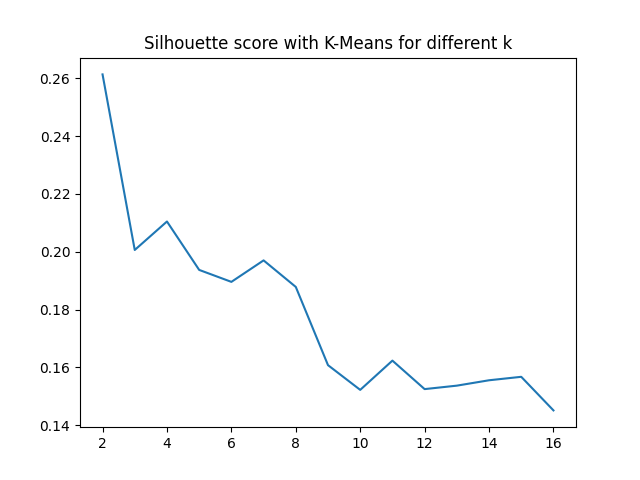
\includegraphics[width=\textwidth]{Imagenes/Bitmap/Clustering/kmeans8sil.png}}%
		\caption{Silhouette Score with K-Means for different $k$}%
		\label{fig:8kmeanssil}
	\end{minipage}
	\hspace{0.4cm}
	\begin{minipage}[b]{0.4\paperwidth}
		\centerline{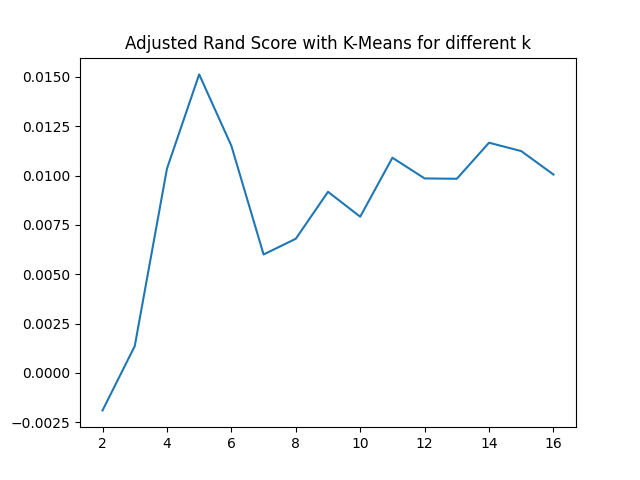
\includegraphics[width=\textwidth]{Imagenes/Bitmap/Clustering/kmeans8ari.png}}%
		\caption{Adjusted Rand Index with K-Means for different $k$}%
		\label{fig:8kmeansari}
	\end{minipage}
\end{figure}

Analysing first Figure \ref{fig:8kmeanssil}, which show us the Silhouette Score for different numbers of clusters, we can observe that its result is very similar to the one represented by the Figure \ref{fig:nkmeanssil}. As in that case, the best Silhouette Score is obtained when the parameter has the value two. However, this result is far from our classification which has twelve different categories (these were defined Section \ref{sect:DatPrep}). This Silhouette Score means that more than two clusters do not differentiate well enough.

To check how the resulting classification fits with our categorisation, we use the Adjusted Rand Index (as it is described in Figure \ref{fig:8kmeansari}). However, the best result that we are able to obtain is with five cluster and its Adjusted Rand Index is around 0.015. As we know, it is a value very close to zero, what means that there are not enough coincidences in the resulting classification and our categorisation. The rest of the values with other numbers of cluster are worst than this.

After this unfortunate results, we are going to carry out the analysis with DBSCAN algorithm. As we have explained, DBSCAN requires a threshold distance and a minimum number of elements that can create a cluster as parameters. As in Section \ref{sect:clust1}, we are going to assign the value of three to this last parameter and to execute with different $\varepsilon$ values (the threshold distance) for the analysis. Furthermore, as it is possible to execute it with different metrics we are going to try with both euclidean and manhattan distance. Then, the Silhouette Score and Adjusted Rand Index of each execution are calculated.

\begin{figure}
	\centering%
	\centerline{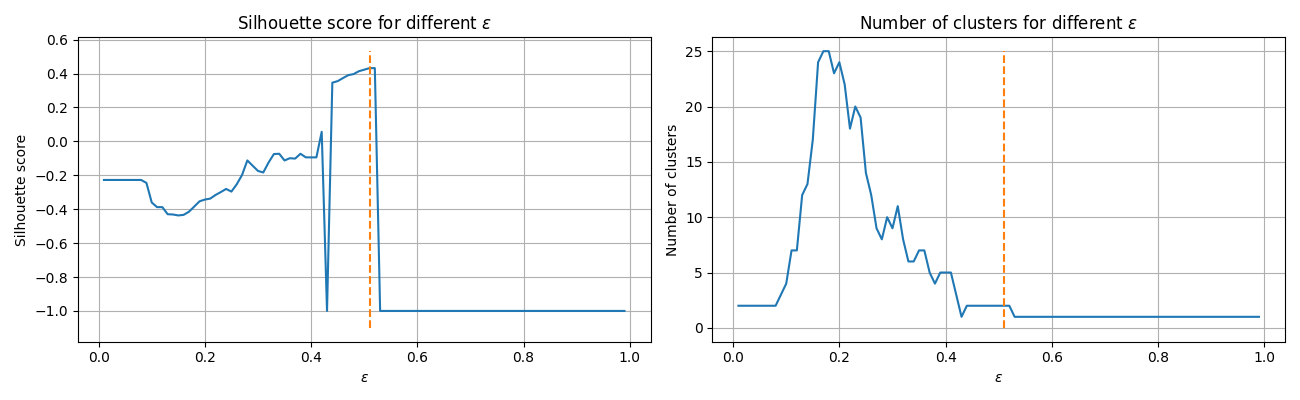
\includegraphics[width=\textwidth]{Imagenes/Bitmap/Clustering/dbscan8sil.png}}%
	\caption{Results of DBSCAN execution with manhattan metric}%
	\label{fig:dbscanman}
\end{figure}

The results of the Silhouette Score calculation with both metrics is very similar. For this reason, we will only show the one with the manhattan distance (see Figure \ref{fig:dbscanman}). In the graph which represent the different Silhouette Score values depending on the taken $\varepsilon$, we are able to see that the maximum value is obtained with a threshold distance that creates two different clusters. As with the K-Means algorithm, indicates that the best differentiating classification is very far from our categorisation. Once we have observed the same result with these two algorithms, we can claim that our different categories are not enough differentiated for the clustering algorithms with the eight selected dimensions.

\begin{figure}[h]
	\centering%
	\centerline{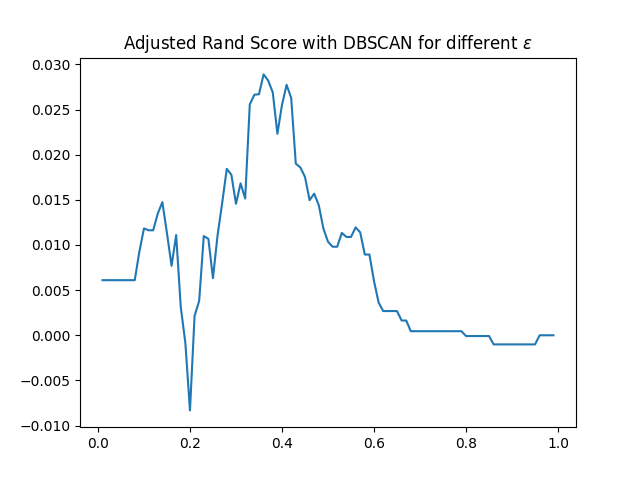
\includegraphics[width=0.5\textwidth]{Imagenes/Bitmap/Clustering/dbscan8ari.png}}%
	\caption{Adjusted Rand Index of DBSCAN with manhattan metric}%
	\label{fig:dbscan8ari}
\end{figure}

As expected, the results of the Adjusted Rand Index are very close to zero again. It can be observed in Figure \ref{fig:dbscan8ari}. The higher Adjusted Rand Index does not achieve the value of 0.03 and the rest of the values are smaller than it. This means that our categorisation does not fit with the returned classification.

In conclusion, the two clustering techniques that we have used for analyse the data with the selected eight dimension do not return a classification similar to that defined by us. However, the results with all features were not initially promising. It could mean that the implemented style markers are not good enough in order to describe the style based on the recipient. Nevertheless, it would be necessary a research with a bigger amount of messages to say that and, perhaps, with a more balanced distribution of each category.